\chapter{Research Proposal}
\label{ch:proposal}

This document previously demonstrated the performance of machine learning on a
set of nuclear material isotopics to calculate a reactor parameter of interest:
burnup.  Additionally, there have been various methods discussed for
understanding the learned model's behavior and thus the quality of the results.
Moving forward to a set of experiments is now possible.

Before describing the experiments, some topics and issues are addressed in
Section \ref{sec:prep}.  Next, the proposed research experimental design is
presented. Sections \ref{sec:exp1}, \ref{sec:exp2}, and \ref{sec:exp3} describe
how this work will probe the viability of statistical learning using direct
isotopic information, information obtained from gamma spectra, and other fuel
cycle flows, respectively.  Discussed separately is the planned implementation
of comparing methods using the Bayesian framework in Section
\ref{sec:modelcompare}. Finally, the timeline of this project is covered in
Section \ref{sec:timeline}.

\section{Experiment Preparations}
\label{sec:prep}

\subsection*{Expanding Training Set}

As identified in Section \ref{sec:valid}, the testing set used for the
demonstration was not suitable for further study without being expanded.  Many
algorithms are developed on an assumption that the training set will be
\gls{i.i.d.}.  This is important so that the model does not overvalue or
overfit a certain area in the training space.  The next step is to provide a
larger, more diverse training set to the algorithms so they can better predict
when faced with new instances. This diversity will be suggested from the
\gls{SFCOMPO} database \cite{sfcompo}, as it includes many common domestic and 
international reactors.

The SFCOMPO-2.0 relational database \cite{sfcompo} has approximately 750
\gls{SNF} measurements from 44 reactors. While this is not sufficient as a
training set, it provides a better framework for simulating a larger training
set using \gls{ORIGEN}.  After cross-validation, diagnostics, and optimization,
the trained models can be tested against the entries in this database to
provide a clear estimate of of the model performance. 

\subsection*{Finalizing Set of Algorithms}

The three algorithms in the demonstration (nearest neighbor, ridge, and support
vector regression) are not necessarily the set that will be evaluated for the
experiments. After these are used to train new models on a larger training set
for comparison, other algorithms can be speedily assessed as well.  Since
support vector-, distance-, and linear-based models are already represented,
other obvious choices include Bayesian methods, decision trees, neural
networks, or ensemble methods \cite{elements_stats}. 

\subsection*{Computational Framework and Resources}

Thus far, all simulations and training have not required more processing than
available on a personal laptop. However, some algorithms do require larger
amounts of computational time (e.g., artifical neural networks).  If necessary,
the training stage can be done using the \gls{CHTC}, which is available to
University of Wisconsin researchers. 

\section[Experiment 1: Direct Isotopics]{Experiment 1\\ 
\large{\textit{Viability of Statistical Learning on Direct Isotopics}}}
\label{sec:exp1}

The first experiment will be a purposefully constructed version of the
demonstration: evaluating the model performance with known isotopics.  This
sheds light on how this methodology will perform on the simplest scenario,
providing an estimate on the maximum level of performance.  \textit{The main
purpose of this experiment is to iteratively probe the usefulness of
statistical methods for determining reactor parameters, ultimately choosing the 
best performing methods.}
\\
\begin{figure}[!htb]
    \centering
    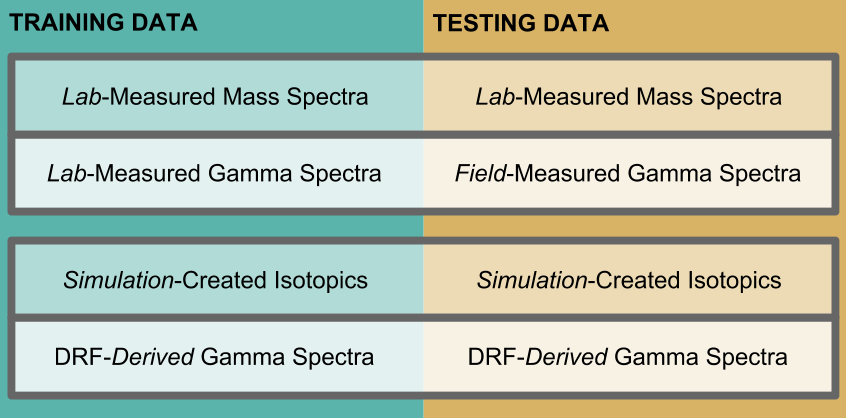
\includegraphics[width=\linewidth]{./chapters/proposal/proposal.png}
    \caption{Physical and Computational Comparisons for Experiments 1 and 2}
    \label{fig:proposal}
\end{figure}

Figure \ref{fig:proposal} shows what type of input can be used for training and
testing (or prediction). The two horizontal boxes are the physical and
computational forms of what these experiments are simulating, respectively. The
lab-measured mass spectra correspond to the perfect information being referred
to here. In the computational context, these measurements instead come from
simulations. Mass spectra results are thus approximated as the direct isotopics
given from the simulations, since mass spectrometry provides highly reliable
and accurate information.

The variables for this experiment will include the following:
\begin{enumerate}
  \itemsep-0.75em
  \item the complexity of the machine learning algorithm used, 
  \item feature reduction, and 
  \item different subsets of the desicion space. 
\end{enumerate}
As previously mentioned, there are complexity differences among the algorithms,
which will be taken into account.  The distance-based nearest neighbor
algorithm is by far the simplest, as it does not do any learning. By contrast,
\gls{SVR} with a radial basis function kernel to work in many dimensions is
much more elaborate.  The feature reduction will be different subsets of
isotopes, e.g., top \textit{n} nuclides, fission products only, etc.  Reducing
the decision space can be done by, e.g., simplifying the regression task by
fixing the reactor type. It is expected that a more complex algorithm (e.g.,
\gls{SVR}) will be needed, and that preprocessing and/or manual feature
reduction will assist in creating higher quality models.  Simplifying the
decision space should always improve prediction, but it is not obvious how much
it will be needed for burnup prediction specifically.

\subsection*{Risks}

It is possible that statistical models trained on direct isotopic information
do not perform well enough.  Other than attempting different types of
algorithms, it is possible to preprocess the data, statistically performing
feature reduction via \gls{PCA}. If this is not sufficient, it is possible
\gls{SNF} is has too many or too few correlated features to provide reliable
models across the space of current reactor technologies. Since separated
plutonium and \gls{UOC} have been also studied using these techniques, it is
possible these materials can provide useable learned models. Additionally, this
methodology would also work if applied to post-detonation materials. There is
work on creating standard materials to represent the ``urban canyon'', so this
is another subject that could benefit from statistical correlations
\cite{refmaterial}.

\section[Experiment 2: Gamma Spectra]{Experiment 2\\ 
\large{\textit{Viability of Statistical Learning on Gamma Spectra}}}
\label{sec:exp2}

The second experiment will be the previously discussed extension of the
demonstration by applying detector response functions to the \gls{SNF}
isotopics: evaluating the model performance with reduced isotopic information.
This demonstrates the usefulness of this methodology in a real-world scenario
where exact isotopics are not always known.   \textit{The main objective of
this experiment is to measure the reduction in statistical model parameter
prediction reliability as the quality of the training information is reduced.}

The two bottom portions of the boxes in Figure \ref{fig:proposal} represent a
more realistic measurement scheme, involving a model trained from gamma
spectrometers rather than the lengthy process of performing mass spectrometry
on the samples.  In the physical context, the measurements for training would
be done using a semiconductor gamma detector, but the testing or prediction
step may be done outside of the lab on a different detector.  This will be
captured by applying different detector response functions to the radionuclide
inventories from the simulations.

The variables for this experiment will include the following:
\begin{enumerate}
  \itemsep-0.75em
  \item the complexity of the machine learning algorithm used, 
  \item feature reduction (implicit), and 
  \item quality of training and/or testing data set.
\end{enumerate}
As in Section \ref{sec:exp1}, the algorithm complexity will be used to explain
performance.  The feature reduction is implicit here, since gamma detection
only includes radionuclides within the \gls{SNF} isotopics. The indirect
isotopic training data are likely going to reduce the prediction capability of
the models, but it is not yet clear if a response function simulating a
hand-held NaI gamma detector can provide any useful predictions.  And while it
is still expected that the complex algorithms will perform better, it is not
yet obvious if different algorithms than the ones used in Experiment 1 will be
needed. 

\subsection*{Risks}

It is possible that statistical models trained on indirect isotopic information
do not perform well enough. Again, here, different algorithms may perform
better than others due to the underlying optimization processes. Further
feature reduction could also prove useful, focusing on particular energy
regions or particular peaks throughout the spectrum. The quality of the
training information can be improved slightly by using an isotope
identification algorithm; this may improve the performance, as they are
developed to automatically report isotopics from gamma spectra. If this still
is not sufficient, it may be that direct isotopic information (i.e., that
obtained from mass spectrometry) is required for reliable statistical models of
\gls{SNF}.  Although preprocessing could also be investigated here, the
materials discussed above may also be more disposed to defined statistical
correlations.

\section[Experiment 3: Other Fuel Cycle Flows]{Experiment 3\\ 
\large{\textit{Viability of Statistical Learning on Other Fuel Cycle Flows}}}
\label{sec:exp3}

There is already nuclear fuel reprocessing in France for \gls{LWR}s, and
possibly in the forseeable future in China with fast breeder reactors.  Given
the existence of reprocessing in fuel cycles, it is important to develop
nuclear forensics capabilities on processed \gls{SNF}. This is presents an
additional prediction challenge because many of the isotopic, chemical, and
elemental signatures are stripped away in the processing. However, there is a
possibility that plutonium isotopes can provide enough information for
characterization, even with reprocessing \cite{pu_discrimination}. Although
Ref. \cite{pu_discrimination} predicts reactor type and enrichment, it is
enough motivation to pursue burnup as well. 

This experiment is intended to repeat those in Sections \ref{sec:exp1} and
\ref{sec:exp2} with an added layer of complexity from the reprocessing by
including mixed-oxide fuel.  It will be carried out using direct isotopics as
in Section \ref{sec:exp1}, with a goal to use indirect information as in
Section \ref{sec:exp2} pending performance. The training data set will also be
simulated using \gls{ORIGEN}.  \textit{The main purpose of this experiment is
to probe the difficulties of reactor parameter prediction when some of the
inputs are from a cyclical nuclear fuel cycle.}

The variables for this experiment will include the following:
\begin{enumerate}
  \itemsep-0.75em
  \item the complexity of the machine learning algorithm used,
  \item quality of training data set, and 
  \item type of preprocessing for feature reduction.
\end{enumerate}
Because of the increased complexity of the training data, it is expected that a
more involved algorithm will be necessary.  The quality of the training data
set will be varied as well as the type of preprocessing tool.  It is not yet
obvious if the feature reduction is absolutely necessary, but it is expected to
drastically improve the accuracy of burnup prediction.  Feature reduction can
be carried out via a range of discriminant, component, or factor analyses.
Multiple studies have demonstrated success with some of these dimensionality
reduction techniques \cite{nicolaou_2006, nicolaou_2009, nicolaou_2014,
robel_2009, pu_discrimination, jones_viz_2014, jones_snf_2014}.  Because
reprocessing mixes streams of material, \gls{PCA} is not expected to perform as
well as \gls{ICA}.

\subsection*{Risks}

It is possible that this framework is not the best approach to understand fuel
cycles with reprocessing. The first action upon poor performance results is to
try more/different preprocessing tools; this may have to include using domain
knowledge to manually reduce the dimensions. As one of the goals within the
nuclear forensics community is to identify new signatures and/or correlated
measurements, this is not desireable but it could still offer interesting
results. Also, some creativity could be applied to find a method that works for
this type of dataset, such as the iterative partial least squares discriminant
analysis used for \gls{UOC} country and source prediction in Refs.
\cite{robel_2009, pu_discrimination}.

\section{Model Comparison}
\label{sec:modelcompare}

It is essential to be able to compare the methods proposed here against each
other, but also against other analagous methods. For example, Experiment 2
(Section \ref{sec:exp2}) aims to predict reactor history values using simulated
gamma spectra, and \gls{INDEPTH} uses gamma spectra as inputs.  These can be
directly compared using the inverse problem structure introduced in Section
\ref{sec:inverse}. An application of Equation \ref{eq:bayes_words} is discussed
further in Section \ref{sec:invcompare}.

However, the Section \ref{sec:invcompare} discussion excluded some detail for
clarity. If the training data set includes uncertainties, the values discussed
will not just be numbers, but probability distributions.  While initially
uncertainties will be ignored for an approximate analysis, they cannot be
ignored for long in the nuclear forensics context. These are quite important
for obtaining some measure of confidence in the solution.  Including the
uncertainty broadens each predicted parameter to a range of probabilities.
These are then analyzed to produce ranges of confidence in the predictions
\cite{bayes_compare}.  The methods for calculating the necessary probability
distributions are outlined below.

Here, we change the meaning of the variables to represent probability
distributions, as in Equation \ref{eq:distrib}.  $C$ is a constant given by the
marginal likelihood, which can be ignored when calculating relative
probabilities, and $\boldsymbol{d}$ and $\boldsymbol{m}$ represent the training
data set and model parameters, respectively. Thus,
$P(\boldsymbol{d}|\boldsymbol{m})$ is the likelihood distribution function,
$P(\boldsymbol{m})$ is the prior probability distribution, and
$P(\boldsymbol{m}|\boldsymbol{d})$ is the posterior probability distribution.
\begin{equation}
\label{eq:distrib}
  P(\boldsymbol{m}|\boldsymbol{d}) = C\ *\
  P(\boldsymbol{d}|\boldsymbol{m})\ *\ P(\boldsymbol{m})
\end{equation}

Mathematically speaking, the distributions are obtained by integrating over the
relevant probability densities.  For example, the prior probability
distribution can be calculated from Equation \ref{eq:rho}, where
$\boldsymbol{m}$ is the range of predicted model parameters, i.e. burnup
values, and $\boldsymbol{d}$ is a set of nuclide vectors. Also, here,
$\rho(\boldsymbol{x}) = \prod_{i} \rho(x_i)$. 
\begin{equation}
\label{eq:rho}
  P(\boldsymbol{m}) = \int_{\boldsymbol{m}} \rho(\boldsymbol{d}) d\boldsymbol{d}
\end{equation}
Similarly, the likelihood distribution function is obtained as in Equation 
\ref{eq:rho-l}.
\begin{equation}
\label{eq:rho-l}
  P(\boldsymbol{d}|\boldsymbol{m}) = \int_{\boldsymbol{d}, \boldsymbol{m}} \rho(\boldsymbol{d}|\boldsymbol{m}) d\boldsymbol{m}
\end{equation}
In practice, however, these functions are not calculated directly. Below, the
methods chosen to estimate the functions in this work are addressed.

\subsection{Estimating Density Functions}

Estimating a probability density function $\rho(x)$ is not a straightforward
task.  One must have a `feel' for the shape of this function to predict a
smooth curve that will represent the probability density over a range of a
parameter.  One estimation method is binning the parameters in the training set
over a given width and tallying up each bin to form a histogram; using some
kernel, Gaussian for example, provides a function that should approximately
follow the shape of the histogram. The shape of the histogram and function may
strongly depend on the bin size, but this can be handled as a separate
optimization step within the sci-kit learn package \cite{scikit}.

As mentioned, the prior probability distributions are given by the model space,
e.g., reactor parameters as predicted from the machine-learned models.  The
above-mentioned method should be utilized to obtain a prior density function
from the range of burnups.  This will not be necessary because the current
design of the training set will provide a flat density function (i.e., uniform
distribution). However, this is not the case in a real-world scenario with
mostly commercial reactor fuel comprising \gls{SNM} inventories around the
world.  This topic will only be investigated if the training data set is
changed. \cite{bayes_compare} Note: This implies the posterior is now only
dependent on the likelihood.

The likelihood function can be obtained by summing the probability densities of
each nuclide vector ($d$) given some predicted model parameter ($m$, e.g., a
burnup prediction) using some algorithm (e.g., nearest neighbor regression).
In essence, this is a large set of forward problems; it is information
including the database of \gls{SNF} recipes, and the known parameter inputs
compared to the model's parameter predictions.  The goal of this step is to
find the \textit{maximum} likelihood, usually carried out in a step called
\gls{MLE}. In this framework, the training phase provides the maximum
likelihood distribution through the use of cross-validation, since the results
are reported as a mean error with a standard deviation (which can be
converted to accuracy for likelihood) \cite{scikit}. 

Unfortunately, \gls{MLE} is not this simple for other methods that do not
employ cross-validation \cite{gentle_bayes, bayes_compare}. This will indeed
have to be broached in order to compare the machine-learned models against
other forensics methods but is beyond the scope of this work.

\subsection{Posterior Odds}

Finally, a non-normalized posterior probability distribution, $P(m_i|d)$, can
be calculated directly from the likelihood and prior distributions. The same
can be done for a model obtained from a different algorithm, $P(m_j|d)$. The
relative posterior probability distribution, aka \textit{posterior odds}
\cite{bayes_compare}, can then be obtained as in Equation \ref{eq:postodds}.
Here, $B_{ij} = \frac{\rho(d|m_i)}{\rho(d|m_j)}$ and is referred to as the
\textit{Bayes factor}.
\begin{equation}
\label{eq:postodds}
  \frac{P(m_i|d)}{P(m_j|d)} = B_{ij} \frac{P(m_i)}{P(m_j)}
\end{equation}

Given relatively uniform priors, the Bayes factor is the key component that
determines relative model performance. Table \ref{tbl:strength}\footnote{This
table is reproduced from Ref. \cite{bayes_compare}.} shows an approximation of
posterior probabilities calculated from $\lvert lnB_{ij} \rvert$. Taking the
logarithm of the Bayes factor is done for convenience, since taking the product
of many likelihoods tends towards zero.

\begin{table}[!hbt]
  \centering
  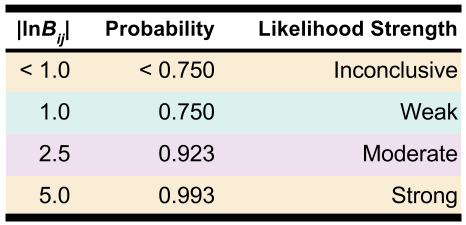
\includegraphics[width=0.8\linewidth]{./chapters/proposal/evidence-strength.png}
  \caption{Model Comparison using Likelihood Strength}
  \label{tbl:strength}
\end{table}

In summary, given a mean-squared error and its standard deviation from using cross-validation 
with any machine learning algorithm, the \gls{MLE} can be formed. To compare two models, a ratio of $\text{MLE}_i$ to $\text{MLE}_j$,
called the posterior odds, provides the probability of model $i$ being correct.


\section{Timeline}
\label{sec:timeline}

oh hi
